% Options for packages loaded elsewhere
\PassOptionsToPackage{unicode}{hyperref}
\PassOptionsToPackage{hyphens}{url}
%
\documentclass[
]{article}
\usepackage{amsmath,amssymb}
\usepackage{lmodern}
\usepackage{ifxetex,ifluatex}
\ifnum 0\ifxetex 1\fi\ifluatex 1\fi=0 % if pdftex
  \usepackage[T1]{fontenc}
  \usepackage[utf8]{inputenc}
  \usepackage{textcomp} % provide euro and other symbols
\else % if luatex or xetex
  \usepackage{unicode-math}
  \defaultfontfeatures{Scale=MatchLowercase}
  \defaultfontfeatures[\rmfamily]{Ligatures=TeX,Scale=1}
\fi
% Use upquote if available, for straight quotes in verbatim environments
\IfFileExists{upquote.sty}{\usepackage{upquote}}{}
\IfFileExists{microtype.sty}{% use microtype if available
  \usepackage[]{microtype}
  \UseMicrotypeSet[protrusion]{basicmath} % disable protrusion for tt fonts
}{}
\makeatletter
\@ifundefined{KOMAClassName}{% if non-KOMA class
  \IfFileExists{parskip.sty}{%
    \usepackage{parskip}
  }{% else
    \setlength{\parindent}{0pt}
    \setlength{\parskip}{6pt plus 2pt minus 1pt}}
}{% if KOMA class
  \KOMAoptions{parskip=half}}
\makeatother
\usepackage{xcolor}
\IfFileExists{xurl.sty}{\usepackage{xurl}}{} % add URL line breaks if available
\IfFileExists{bookmark.sty}{\usepackage{bookmark}}{\usepackage{hyperref}}
\hypersetup{
  hidelinks,
  pdfcreator={LaTeX via pandoc}}
\urlstyle{same} % disable monospaced font for URLs
\usepackage[margin=1in]{geometry}
\usepackage{color}
\usepackage{fancyvrb}
\newcommand{\VerbBar}{|}
\newcommand{\VERB}{\Verb[commandchars=\\\{\}]}
\DefineVerbatimEnvironment{Highlighting}{Verbatim}{commandchars=\\\{\}}
% Add ',fontsize=\small' for more characters per line
\usepackage{framed}
\definecolor{shadecolor}{RGB}{248,248,248}
\newenvironment{Shaded}{\begin{snugshade}}{\end{snugshade}}
\newcommand{\AlertTok}[1]{\textcolor[rgb]{0.94,0.16,0.16}{#1}}
\newcommand{\AnnotationTok}[1]{\textcolor[rgb]{0.56,0.35,0.01}{\textbf{\textit{#1}}}}
\newcommand{\AttributeTok}[1]{\textcolor[rgb]{0.77,0.63,0.00}{#1}}
\newcommand{\BaseNTok}[1]{\textcolor[rgb]{0.00,0.00,0.81}{#1}}
\newcommand{\BuiltInTok}[1]{#1}
\newcommand{\CharTok}[1]{\textcolor[rgb]{0.31,0.60,0.02}{#1}}
\newcommand{\CommentTok}[1]{\textcolor[rgb]{0.56,0.35,0.01}{\textit{#1}}}
\newcommand{\CommentVarTok}[1]{\textcolor[rgb]{0.56,0.35,0.01}{\textbf{\textit{#1}}}}
\newcommand{\ConstantTok}[1]{\textcolor[rgb]{0.00,0.00,0.00}{#1}}
\newcommand{\ControlFlowTok}[1]{\textcolor[rgb]{0.13,0.29,0.53}{\textbf{#1}}}
\newcommand{\DataTypeTok}[1]{\textcolor[rgb]{0.13,0.29,0.53}{#1}}
\newcommand{\DecValTok}[1]{\textcolor[rgb]{0.00,0.00,0.81}{#1}}
\newcommand{\DocumentationTok}[1]{\textcolor[rgb]{0.56,0.35,0.01}{\textbf{\textit{#1}}}}
\newcommand{\ErrorTok}[1]{\textcolor[rgb]{0.64,0.00,0.00}{\textbf{#1}}}
\newcommand{\ExtensionTok}[1]{#1}
\newcommand{\FloatTok}[1]{\textcolor[rgb]{0.00,0.00,0.81}{#1}}
\newcommand{\FunctionTok}[1]{\textcolor[rgb]{0.00,0.00,0.00}{#1}}
\newcommand{\ImportTok}[1]{#1}
\newcommand{\InformationTok}[1]{\textcolor[rgb]{0.56,0.35,0.01}{\textbf{\textit{#1}}}}
\newcommand{\KeywordTok}[1]{\textcolor[rgb]{0.13,0.29,0.53}{\textbf{#1}}}
\newcommand{\NormalTok}[1]{#1}
\newcommand{\OperatorTok}[1]{\textcolor[rgb]{0.81,0.36,0.00}{\textbf{#1}}}
\newcommand{\OtherTok}[1]{\textcolor[rgb]{0.56,0.35,0.01}{#1}}
\newcommand{\PreprocessorTok}[1]{\textcolor[rgb]{0.56,0.35,0.01}{\textit{#1}}}
\newcommand{\RegionMarkerTok}[1]{#1}
\newcommand{\SpecialCharTok}[1]{\textcolor[rgb]{0.00,0.00,0.00}{#1}}
\newcommand{\SpecialStringTok}[1]{\textcolor[rgb]{0.31,0.60,0.02}{#1}}
\newcommand{\StringTok}[1]{\textcolor[rgb]{0.31,0.60,0.02}{#1}}
\newcommand{\VariableTok}[1]{\textcolor[rgb]{0.00,0.00,0.00}{#1}}
\newcommand{\VerbatimStringTok}[1]{\textcolor[rgb]{0.31,0.60,0.02}{#1}}
\newcommand{\WarningTok}[1]{\textcolor[rgb]{0.56,0.35,0.01}{\textbf{\textit{#1}}}}
\usepackage{longtable,booktabs,array}
\usepackage{calc} % for calculating minipage widths
% Correct order of tables after \paragraph or \subparagraph
\usepackage{etoolbox}
\makeatletter
\patchcmd\longtable{\par}{\if@noskipsec\mbox{}\fi\par}{}{}
\makeatother
% Allow footnotes in longtable head/foot
\IfFileExists{footnotehyper.sty}{\usepackage{footnotehyper}}{\usepackage{footnote}}
\makesavenoteenv{longtable}
\usepackage{graphicx}
\makeatletter
\def\maxwidth{\ifdim\Gin@nat@width>\linewidth\linewidth\else\Gin@nat@width\fi}
\def\maxheight{\ifdim\Gin@nat@height>\textheight\textheight\else\Gin@nat@height\fi}
\makeatother
% Scale images if necessary, so that they will not overflow the page
% margins by default, and it is still possible to overwrite the defaults
% using explicit options in \includegraphics[width, height, ...]{}
\setkeys{Gin}{width=\maxwidth,height=\maxheight,keepaspectratio}
% Set default figure placement to htbp
\makeatletter
\def\fps@figure{htbp}
\makeatother
\setlength{\emergencystretch}{3em} % prevent overfull lines
\providecommand{\tightlist}{%
  \setlength{\itemsep}{0pt}\setlength{\parskip}{0pt}}
\setcounter{secnumdepth}{-\maxdimen} % remove section numbering
\ifluatex
  \usepackage{selnolig}  % disable illegal ligatures
\fi

\author{}
\date{\vspace{-2.5em}}

\begin{document}

\hypertarget{integer-linear-programming-for-systematic-conservation-planning}{%
\section{Integer Linear Programming for Systematic Conservation
Planning}\label{integer-linear-programming-for-systematic-conservation-planning}}

author: Frankie Cho date: 12 November 2021 autosize: true Sustainable
Landscapes Group, UQ

\hypertarget{what-this-skills-training-will-be-about}{%
\section{What this skills training will be
about}\label{what-this-skills-training-will-be-about}}

\begin{itemize}
\tightlist
\item
  What are ILPs?
\item
  Reading the math formulae of an ILP
\item
  Setting up and solving the ILP in Gurobi
\item
  Integer constraints
\item
  Facilitating connectivity
\end{itemize}

\hypertarget{what-are-linear-programs}{%
\section{What are Linear Programs?}\label{what-are-linear-programs}}

Asking a computer to make decisions! - Problem: many many possible
options (combination of actions across space) - Objective: how ``good''
a decision is - Constraints: defines the set of possible decisions --
what you can and can't do

\hypertarget{applications-of-lp-ilp}{%
\section{Applications of LP/ ILP}\label{applications-of-lp-ilp}}

\begin{itemize}
\tightlist
\item
  Conservation decision making
\item
  Transportation/ facility location problems
\item
  Network flow and optimization
\item
  Scheduling
\item
  Design markets (e.g.~auctions, fixed-price payments)
\end{itemize}

\hypertarget{why-do-we-need-linear-programs}{%
\section{Why do we need Linear
Programs?}\label{why-do-we-need-linear-programs}}

class: small-code Consider a decision problem of choosing 25\% of
locations out of \(N\) locations for conservation.

Each location is either ``chosen'' or ``not chosen'' (0 or 1).

\begin{Shaded}
\begin{Highlighting}[]
\FunctionTok{source}\NormalTok{(}\StringTok{\textquotesingle{}ilp{-}intro{-}functions.R\textquotesingle{}}\NormalTok{)}
\NormalTok{N }\OtherTok{\textless{}{-}} \FunctionTok{c}\NormalTok{(}\DecValTok{20}\NormalTok{,}\DecValTok{80}\NormalTok{,}\DecValTok{100}\NormalTok{,}\DecValTok{1000}\NormalTok{)}
\NormalTok{nchoosek }\OtherTok{\textless{}{-}} \ControlFlowTok{function}\NormalTok{(n) }\FunctionTok{choose}\NormalTok{(n, n}\SpecialCharTok{/}\DecValTok{4}\NormalTok{)}
\NormalTok{Combinations }\OtherTok{\textless{}{-}} \FunctionTok{sapply}\NormalTok{(N, nchoosek)}
\FunctionTok{kable}\NormalTok{(}\FunctionTok{data.frame}\NormalTok{(N, Combinations))}
\end{Highlighting}
\end{Shaded}

\begin{longtable}[]{@{}rr@{}}
\toprule
N & Combinations \\
\midrule
\endhead
20 & 1.550400e+04 \\
80 & 3.535316e+18 \\
100 & 2.425193e+23 \\
1000 & 4.822840e+242 \\
\bottomrule
\end{longtable}

How to search through these combinations efficiently?

\hypertarget{why-linear-programming}{%
\section{Why Linear Programming?}\label{why-linear-programming}}

Compared to simulated annealing based methods ILP offers: - Known
solution quality (known gap to optimality) - Shorter computation time -
Cross-disciplinary: immediately benefit from latest models/ software in
operations research \& maths instead of waiting for it to
``trickle-down'' to your domain

\hypertarget{what-data-do-we-need}{%
\section{What data do we need?}\label{what-data-do-we-need}}

\begin{enumerate}
\def\labelenumi{\alph{enumi})}
\item
  Data for the objective function
\item
  Data for the constraints
\item
  List of variables we ``allow'' the computer to choose
\end{enumerate}

\hypertarget{example-planning-for-reserve-sites}{%
\subsubsection{Example: Planning for reserve
sites}\label{example-planning-for-reserve-sites}}

\begin{enumerate}
\def\labelenumi{\alph{enumi})}
\item
  Raster of the costs of reserve sites
\item
  Raster of species distribution, spatial connectivity matrix
\item
  Binary decision variable: whether a reserve site is ``selected'' in
  the location
\end{enumerate}

\hypertarget{possible-ilp-formulations}{%
\section{Possible ILP formulations}\label{possible-ilp-formulations}}

\begin{enumerate}
\def\labelenumi{\arabic{enumi}.}
\tightlist
\item
  Minimise cost while constraining biodiversity goals
\item
  Maximise biodiversity goals while keeping a budget
\end{enumerate}

\begin{center}\rule{0.5\linewidth}{0.5pt}\end{center}

\begin{figure}
\centering
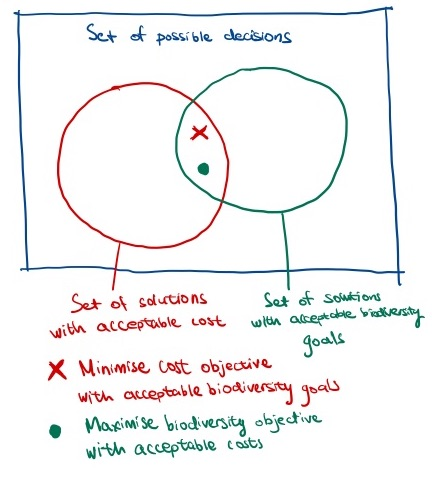
\includegraphics{images/Systematic Conservation Planning -2.jpeg}
\caption{alt text}
\end{figure}

\hypertarget{code-example-cost-minimization-problem}{%
\section{Code example: cost minimization
problem}\label{code-example-cost-minimization-problem}}

\begin{itemize}
\tightlist
\item
  Objective: Minimize total cost of conservation
\item
  Constraint: Protect 25\% of the population present in this habitat
  (goal)
\end{itemize}

\hypertarget{code-example-cost-minimization-problem-1}{%
\section{Code example: cost minimization
problem}\label{code-example-cost-minimization-problem-1}}

class: small-code

\begin{Shaded}
\begin{Highlighting}[]
\FunctionTok{library}\NormalTok{(ggplot2)}
\FunctionTok{library}\NormalTok{(reshape2)}
\FunctionTok{library}\NormalTok{(ggpubr)}

\FunctionTok{set.seed}\NormalTok{(}\DecValTok{123}\NormalTok{)}
\NormalTok{nx }\OtherTok{\textless{}{-}} \DecValTok{50}
\NormalTok{ny }\OtherTok{\textless{}{-}} \DecValTok{50}
\NormalTok{N  }\OtherTok{\textless{}{-}}\NormalTok{ nx}\SpecialCharTok{*}\NormalTok{ny}
\NormalTok{r1 }\OtherTok{\textless{}{-}} \FunctionTok{matrix}\NormalTok{(}\FunctionTok{rpois}\NormalTok{(nx}\SpecialCharTok{*}\NormalTok{ny, }\FunctionTok{correlatedSpatialGrid}\NormalTok{(.}\DecValTok{5}\NormalTok{,nx,ny)), }\AttributeTok{ncol =}\NormalTok{ ny, }\AttributeTok{nrow =}\NormalTok{ nx)}
\NormalTok{r2 }\OtherTok{\textless{}{-}} \FunctionTok{matrix}\NormalTok{(}\FunctionTok{rpois}\NormalTok{(nx}\SpecialCharTok{*}\NormalTok{ny, }\FunctionTok{correlatedSpatialGrid}\NormalTok{(}\DecValTok{2}\NormalTok{,nx,ny)), }\AttributeTok{ncol =}\NormalTok{ ny, }\AttributeTok{nrow =}\NormalTok{ nx)}
\NormalTok{c  }\OtherTok{\textless{}{-}} \FunctionTok{matrix}\NormalTok{(}\FunctionTok{exp}\NormalTok{(}\FunctionTok{rnorm}\NormalTok{(}\FunctionTok{correlatedSpatialGrid}\NormalTok{(}\DecValTok{5}\NormalTok{,nx,ny), }\DecValTok{0}\NormalTok{)), }\AttributeTok{ncol =}\NormalTok{ ny, }\AttributeTok{nrow =}\NormalTok{ nx)}
\NormalTok{plotR1 }\OtherTok{\textless{}{-}} \FunctionTok{plotSpatialGrid}\NormalTok{(r1, }\AttributeTok{label =} \StringTok{"Species 1"}\NormalTok{, }\AttributeTok{colorScheme =} \StringTok{\textquotesingle{}viridis\textquotesingle{}}\NormalTok{)}
\NormalTok{plotR2 }\OtherTok{\textless{}{-}} \FunctionTok{plotSpatialGrid}\NormalTok{(r2, }\AttributeTok{label =} \StringTok{"Species 2"}\NormalTok{, }\AttributeTok{colorScheme =} \StringTok{\textquotesingle{}viridis\textquotesingle{}}\NormalTok{)}
\NormalTok{plotC  }\OtherTok{\textless{}{-}} \FunctionTok{plotSpatialGrid}\NormalTok{(c, }\AttributeTok{label =} \StringTok{"Cost"}\NormalTok{, }\AttributeTok{colorScheme =} \StringTok{\textquotesingle{}magma\textquotesingle{}}\NormalTok{)}
\NormalTok{ggpubr}\SpecialCharTok{::}\FunctionTok{ggarrange}\NormalTok{(plotR1, plotR2, plotC, }\AttributeTok{nrow =} \DecValTok{1}\NormalTok{)}
\end{Highlighting}
\end{Shaded}

\hypertarget{reserve-selection-problem}{%
\section{Reserve Selection Problem}\label{reserve-selection-problem}}

left: 70\%

\[ \min_\mathbf{x} \sum^N_{i=1} c_i x_i \: (1) \]
\[ s.t. \sum_{i=1}^N r_{ik} x_i \geq T_k, \forall k \in K \: (2) \]
\[ x_i \in \{0,1\} \: (3) \]

How to use these formulations in my own problem??

We need to find \textbf{data} variables and \textbf{decision} variables

\begin{center}\rule{0.5\linewidth}{0.5pt}\end{center}

\begin{enumerate}
\def\labelenumi{\arabic{enumi}.}
\tightlist
\item
  Objective function
\item
  Linear constraints
\item
  Bound constraints
\end{enumerate}

\hypertarget{components-of-the-problem}{%
\section{Components of the problem}\label{components-of-the-problem}}

title: false \#\#\# Our problem \(N= 2500\): 2500` possible locations to
choose from

\(K=2\): two species we are concerned about

\hypertarget{data-we-give-to-the-problem}{%
\subsubsection{Data we give to the
problem}\label{data-we-give-to-the-problem}}

\(\mathbf{c} = [c_1, c_2, ..., c_N]\) : vector of length N, costs of
setting up a reserve at each location

\(\mathbf{r}_k = [r_{1k}, r_{2k}, ..., r_{Nk}]\) : vector of length N,
number of the species \(k\) in each location -- we have \(K\) number of
these vectors

\(T_k\): a scalar, conservation objective for each species

\hypertarget{gurobi-figures-out-decision-variable}{%
\subsubsection{Gurobi figures out (decision
variable)}\label{gurobi-figures-out-decision-variable}}

\(\mathbf{x} = [x_1, x_2, ..., x_N]\) : vector of length N

Gurobi find the vector \(\mathbf{x}\) that optimises the objective
function

\hypertarget{how-to-tell-between-decision-variables-and-data-variables}{%
\section{How to tell between decision variables and data
variables?}\label{how-to-tell-between-decision-variables-and-data-variables}}

In an LP/ ILP/ MILP, a decision variable cannot be multiplied with
another decision variable

e.g.~\(x_ix_j\) is not feasible in the LP -- if two decision variables
are multiplied together, then the problem will be a quadratic program
(QP) -- computationally intensive

Beyer et al.~(2016) overcomes this problem with `linearization' -- using
another integer variable to represent binary variables multiplied
together

Data variables can multiply with other data variables. Multiplication
occurs before the problem is solved.

\hypertarget{set-notation-for-decision-variables}{%
\section{Set notation for decision
variables}\label{set-notation-for-decision-variables}}

Decision variables need to lie in a \textbf{set}. This describes the
range of values these decision variables can take. \#\#\# Real numbers
\(x_i \in \mathbb{R}\): \(x_i\) can be any real number

\hypertarget{intervals}{%
\subsubsection{Intervals}\label{intervals}}

\(x_i \in [0,1]\) : \(x_i\) is \textbf{between} 0 and 1; can be
non-integer; same as: \(0 \leq x_i \leq 1\)

\hypertarget{integers}{%
\subsubsection{Integers}\label{integers}}

\(x_i \in \{0,1\}\) : \(x_i\) is \textbf{either} 0 or 1 (i.e.~integer)

\(x_i \in \mathbb{Z}\): \(x_i\) must be an integer

\(x_i \in \mathbb{Z}^+\): \(x_i\) must be a positive integer

\hypertarget{why-bother-with-matrix-notation}{%
\section{Why bother with matrix
notation??}\label{why-bother-with-matrix-notation}}

Gurobi accepts problems in the following form:

\[
\min_\mathbf{x} \mathbf{c'x} \\
s.t. \mathbf{A'x} \leq \mathbf{b}
\]

\hypertarget{linear-algebra}{%
\section{Linear algebra}\label{linear-algebra}}

Vector-by-vector multiplication \(\mathbf{c'x}\)

\[
\begin{bmatrix}
c_1 & c_2
\end{bmatrix}
\begin{bmatrix}
x_1 \\
x_2
\end{bmatrix}
=
c_1x_1 + c_2x_2
\]

Matrix-by-vector multiplication \(\mathbf{A'x}\leq b\)

\[
\begin{bmatrix}
r_{1,1} & r_{2,1} \\
r_{1,2} & r_{2,2}
\end{bmatrix}
\begin{bmatrix}
x_1 \\
x_2
\end{bmatrix}
=
\begin{bmatrix}
r_{1,1}x_1 + r_{2,1}x_1 \\
r_{1,2}x_2 + r_{2,2}x_2
\end{bmatrix}
< 
\begin{bmatrix}
T_1 \\
T_2
\end{bmatrix}
\]

\hypertarget{from-matrices-to-gurobi}{%
\section{From matrices to Gurobi}\label{from-matrices-to-gurobi}}

class: small-code title: false

\texttt{result\ \textless{}-\ gurobi(model,\ params)}

\hypertarget{input}{%
\subsection{Input}\label{input}}

\texttt{model\$obj} : \(\mathbf{c}\)

\texttt{model\$A} : \(\mathbf{A}\)

\texttt{model\$rhs} : \(\mathbf{b}\)

\texttt{model\$modelsense} : \(\min\)

\texttt{model\$sense} : \(<\)

\hypertarget{output}{%
\subsection{Output}\label{output}}

\texttt{result\$x} : \(\mathbf{x}\)

\texttt{result\$objval} : \(\mathbf{c'x}\)

\hypertarget{equivalent-formulations-side-by-side}{%
\section{Equivalent formulations
side-by-side}\label{equivalent-formulations-side-by-side}}

title: false \[ \min_\mathbf{x} \sum^N_{i=1} c_i x_i \: (1) \]
\[ s.t. \sum_{i=1}^N r_{ik} x_i \geq T_k, \forall k \in K \: (2) \]
\[ x_i \in \{0,1\} \: (3) \]

Equivalent matrix formulation: \[ \min_\mathbf{x} \mathbf{c'x}\: (1) \]
\[ s.t. \mathbf{r}_k' \mathbf{x} \geq T_k, \forall k \in K \: (2) \]
\[ \mathbf{x} \in \{0,1\} \: (3) \]

\hypertarget{solve-the-problem}{%
\section{Solve the problem}\label{solve-the-problem}}

class: small-code

\begin{Shaded}
\begin{Highlighting}[]
\FunctionTok{library}\NormalTok{(gurobi)}
\NormalTok{model }\OtherTok{\textless{}{-}} \FunctionTok{list}\NormalTok{()}
\NormalTok{model}\SpecialCharTok{$}\NormalTok{obj }\OtherTok{\textless{}{-}} \FunctionTok{as.vector}\NormalTok{(c)}
\NormalTok{model}\SpecialCharTok{$}\NormalTok{modelsense }\OtherTok{\textless{}{-}} \StringTok{\textquotesingle{}min\textquotesingle{}}
\NormalTok{model}\SpecialCharTok{$}\NormalTok{A   }\OtherTok{\textless{}{-}} \FunctionTok{matrix}\NormalTok{(}\FunctionTok{c}\NormalTok{(}\FunctionTok{as.vector}\NormalTok{(r1), }\FunctionTok{as.vector}\NormalTok{(r2)), }\AttributeTok{nrow =} \DecValTok{2}\NormalTok{, }\AttributeTok{byrow =}\NormalTok{ T)}
\NormalTok{model}\SpecialCharTok{$}\NormalTok{rhs }\OtherTok{\textless{}{-}} \FunctionTok{c}\NormalTok{(}\FloatTok{0.25}\SpecialCharTok{*}\FunctionTok{sum}\NormalTok{(r1),}\FloatTok{0.25}\SpecialCharTok{*}\FunctionTok{sum}\NormalTok{(r2))}
\NormalTok{model}\SpecialCharTok{$}\NormalTok{sense }\OtherTok{\textless{}{-}} \StringTok{\textquotesingle{}\textgreater{}\textquotesingle{}}
\NormalTok{model}\SpecialCharTok{$}\NormalTok{vtype }\OtherTok{\textless{}{-}} \StringTok{\textquotesingle{}B\textquotesingle{}}
\NormalTok{result }\OtherTok{\textless{}{-}} \FunctionTok{gurobi}\NormalTok{(model, }\FunctionTok{list}\NormalTok{())}

\NormalTok{plotX }\OtherTok{\textless{}{-}} \FunctionTok{plotSpatialGrid}\NormalTok{(}\FunctionTok{matrix}\NormalTok{(result}\SpecialCharTok{$}\NormalTok{x, }\AttributeTok{ncol =}\NormalTok{ ny, }\AttributeTok{nrow =}\NormalTok{ nx), }\StringTok{\textquotesingle{}Decision\textquotesingle{}}\NormalTok{, }\StringTok{\textquotesingle{}viridis\textquotesingle{}}\NormalTok{)}
\FunctionTok{ggarrange}\NormalTok{(plotC, plotR1, plotR2, plotX, }\AttributeTok{nrow =} \DecValTok{1}\NormalTok{)}
\end{Highlighting}
\end{Shaded}

\hypertarget{improving-the-model}{%
\section{Improving the model?}\label{improving-the-model}}

\begin{enumerate}
\def\labelenumi{\arabic{enumi}.}
\tightlist
\item
  Improving performance by removing integer constraints?
\item
  Spatial connectivity?
\end{enumerate}

\hypertarget{integer-lp-mixed-integer-lp}{%
\section{Integer LP? Mixed-Integer
LP?}\label{integer-lp-mixed-integer-lp}}

\begin{itemize}
\tightlist
\item
  LP allows for non-integer decision variable
\item
  ILP: all decision variables are constrained to be integers (NP-hard)
\item
  MILP: some decision variables continuous, others constrained to be
  integers
\item
  Mixed-Integer LP most common in LP
\item
  Why does your problem need integer constraints?
\item
  Effect on performance
\end{itemize}

\hypertarget{improving-performance-are-integer-constraints-necessary-for-your-problem}{%
\section{Improving performance: are integer constraints necessary for
your
problem?}\label{improving-performance-are-integer-constraints-necessary-for-your-problem}}

class: small-code

LP solves much quicker than ILP/ MILP because it takes advantages of
more efficient algorithms.

\begin{Shaded}
\begin{Highlighting}[]
\NormalTok{start\_time\_integer }\OtherTok{\textless{}{-}} \FunctionTok{Sys.time}\NormalTok{()}
\NormalTok{integer\_result }\OtherTok{\textless{}{-}} \FunctionTok{gurobi}\NormalTok{(model, }\FunctionTok{list}\NormalTok{())}
\NormalTok{end\_time\_integer }\OtherTok{\textless{}{-}} \FunctionTok{Sys.time}\NormalTok{()}

\NormalTok{model\_cont }\OtherTok{\textless{}{-}}\NormalTok{ model}
\NormalTok{model\_cont}\SpecialCharTok{$}\NormalTok{vtype }\OtherTok{\textless{}{-}} \StringTok{\textquotesingle{}C\textquotesingle{}}
\NormalTok{model\_cont}\SpecialCharTok{$}\NormalTok{lb    }\OtherTok{\textless{}{-}} \FunctionTok{rep}\NormalTok{(}\DecValTok{0}\NormalTok{,nx}\SpecialCharTok{*}\NormalTok{ny)}
\NormalTok{model\_cont}\SpecialCharTok{$}\NormalTok{ub    }\OtherTok{\textless{}{-}} \FunctionTok{rep}\NormalTok{(}\DecValTok{1}\NormalTok{,nx}\SpecialCharTok{*}\NormalTok{ny)}
\NormalTok{start\_time\_cont }\OtherTok{\textless{}{-}} \FunctionTok{Sys.time}\NormalTok{()}
\NormalTok{non\_integer\_result }\OtherTok{\textless{}{-}} \FunctionTok{gurobi}\NormalTok{(model\_cont, }\FunctionTok{list}\NormalTok{())}
\NormalTok{end\_time\_cont }\OtherTok{\textless{}{-}} \FunctionTok{Sys.time}\NormalTok{()}

\NormalTok{integer\_time }\OtherTok{\textless{}{-}}\NormalTok{ end\_time\_integer }\SpecialCharTok{{-}}\NormalTok{ start\_time\_integer}
\NormalTok{cont\_time    }\OtherTok{\textless{}{-}}\NormalTok{ end\_time\_cont    }\SpecialCharTok{{-}}\NormalTok{ start\_time\_cont}
\end{Highlighting}
\end{Shaded}

\begin{Shaded}
\begin{Highlighting}[]
\NormalTok{integer\_time}
\end{Highlighting}
\end{Shaded}

\begin{verbatim}
Time difference of 0.01822996 secs
\end{verbatim}

\begin{Shaded}
\begin{Highlighting}[]
\NormalTok{cont\_time}
\end{Highlighting}
\end{Shaded}

\begin{verbatim}
Time difference of 0.006899118 secs
\end{verbatim}

\hypertarget{integer-relaxation-results}{%
\section{Integer relaxation --
results}\label{integer-relaxation-results}}

title: false class: small-code

Some LP will lead to integer results even when integer constraints are
not explicitly imposed. Investigate why integer constraints are needed
for your problem.

\begin{Shaded}
\begin{Highlighting}[]
\NormalTok{plotXInt }\OtherTok{\textless{}{-}} \FunctionTok{plotSpatialGrid}\NormalTok{(}\FunctionTok{matrix}\NormalTok{(integer\_result}\SpecialCharTok{$}\NormalTok{x, }\AttributeTok{ncol =}\NormalTok{ ny, }\AttributeTok{nrow =}\NormalTok{ nx), }\StringTok{\textquotesingle{}Decision (integer)\textquotesingle{}}\NormalTok{, }\StringTok{\textquotesingle{}viridis\textquotesingle{}}\NormalTok{)}
\NormalTok{plotXCont }\OtherTok{\textless{}{-}} \FunctionTok{plotSpatialGrid}\NormalTok{(}\FunctionTok{matrix}\NormalTok{(non\_integer\_result}\SpecialCharTok{$}\NormalTok{x, }\AttributeTok{ncol =}\NormalTok{ ny, }\AttributeTok{nrow =}\NormalTok{ nx), }\StringTok{\textquotesingle{}Decision (continuous)\textquotesingle{}}\NormalTok{, }\StringTok{\textquotesingle{}viridis\textquotesingle{}}\NormalTok{)}
\FunctionTok{ggarrange}\NormalTok{(plotX, plotXCont, }\AttributeTok{nrow=}\DecValTok{1}\NormalTok{);}
\end{Highlighting}
\end{Shaded}

\hypertarget{spatial-connectivity}{%
\section{Spatial connectivity}\label{spatial-connectivity}}

\begin{itemize}
\tightlist
\item
  Even though species distribution and costs are spatially correlated,
  the sites selected weren't
\item
  Penalties for spatial fragmentation?
\end{itemize}

\hypertarget{rewarding-spatially-connected-solutions-in-the-objective}{%
\section{Rewarding spatially-connected solutions in the
objective}\label{rewarding-spatially-connected-solutions-in-the-objective}}

\[
\min_{\mathbf{x}} \sum_{i=1}^N c_ix_i - b \sum_{i=1}^N \sum_{j=1}^N z_{ij} \\
s.t. - x_i + z_{ij} \leq 0  \: \forall (i,j) \in E \\
- x_j + z_{ij} \leq 0  \:  \forall (i,j) \in E \\
- x_i - x_j + z_{ij} \geq -1  \:  \forall (i,j) \in E
\]

This ensured that for neighbours \(i\) and \(j\), if both \(x_i\) and
\(x_j\) are equal to \(1\), then \(z_{ij}\) must be 1. Otherwise,
\(z_{ij} = 0\). In other words \(z_{ij}\) replaced \(x_ix_j\).

Notice the increase in number of constraints! (increase by number of
elements in \(E\) times 3)

\hypertarget{weighting-factor}{%
\section{Weighting factor}\label{weighting-factor}}

\begin{itemize}
\tightlist
\item
  \(b\): controls relative weighting between multiple objectives
\item
  If \(b\) is small, then the first objective (minimising cost) is more
  important
\item
  If \(b\) is large, then the second objective (spatial connectivity) is
  more important
\item
  Researcher solves problems by iterating values of \(b\)
\item
  Set of solutions where you cannot improve one objective without doing
  worse in another objective
\end{itemize}

\begin{center}\rule{0.5\linewidth}{0.5pt}\end{center}

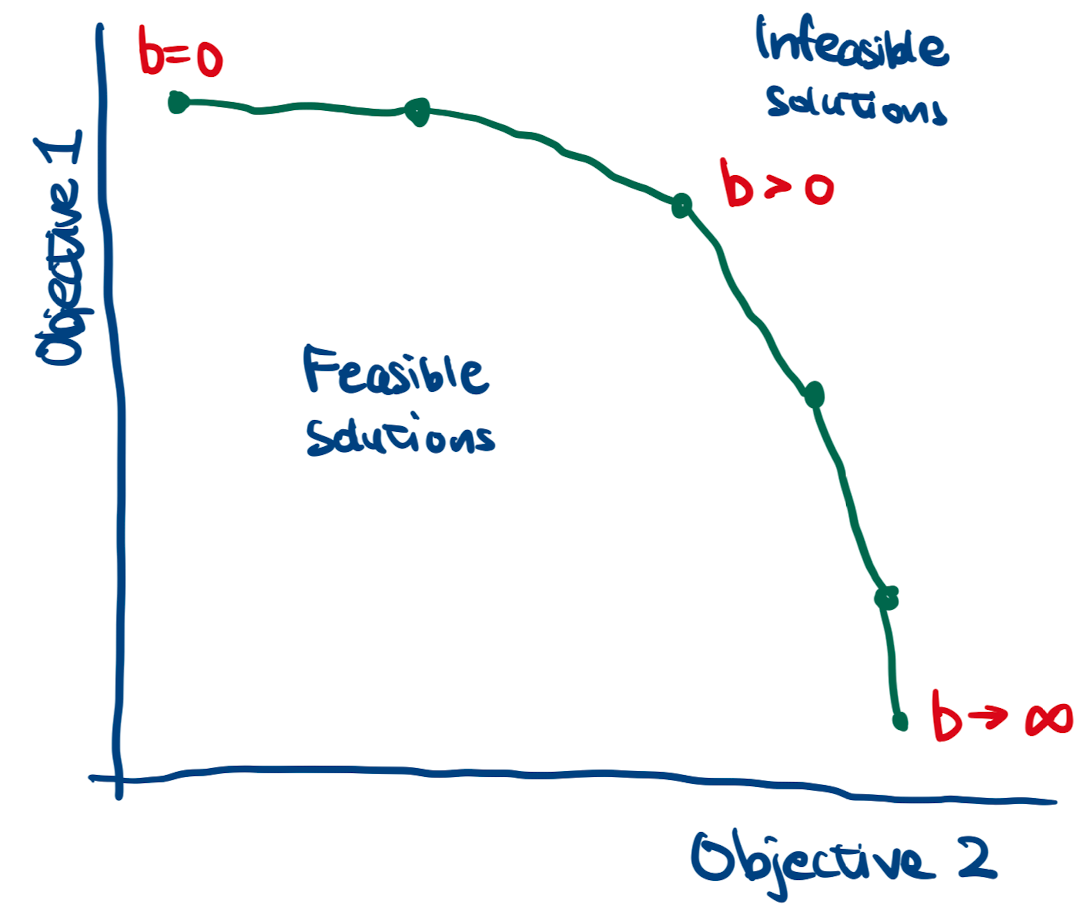
\includegraphics{images/tradeoff.png} ``Efficiency frontier'' aka:
``Pareto frontier'', ``Trade-off curves''

\hypertarget{set-up-a-constraint-matrix}{%
\section{Set up a constraint matrix}\label{set-up-a-constraint-matrix}}

class: small-code Possible to alter the spatial connectivity in result
through a linearised objective

\begin{Shaded}
\begin{Highlighting}[]
\NormalTok{W }\OtherTok{\textless{}{-}} \FunctionTok{spatialWeightsMatrix}\NormalTok{(nx, ny, }\AttributeTok{rowStandardise =} \ConstantTok{FALSE}\NormalTok{)}
\NormalTok{W[}\FunctionTok{lower.tri}\NormalTok{(W)] }\OtherTok{\textless{}{-}} \DecValTok{0} \CommentTok{\# Set it as a upper triangular matrix}
\NormalTok{E }\OtherTok{\textless{}{-}} \FunctionTok{which}\NormalTok{(W}\SpecialCharTok{!=}\DecValTok{0}\NormalTok{, }\AttributeTok{arr.ind =} \ConstantTok{TRUE}\NormalTok{) }\CommentTok{\# Get set of neighbours E, with two columns, one for index of i and one for index of j}
\NormalTok{num\_neighbours }\OtherTok{\textless{}{-}} \FunctionTok{nrow}\NormalTok{(E)}
\NormalTok{A\_r1 }\OtherTok{\textless{}{-}} \FunctionTok{c}\NormalTok{(}\FunctionTok{as.vector}\NormalTok{(r1), }\FunctionTok{rep}\NormalTok{(}\DecValTok{0}\NormalTok{, num\_neighbours))}
\NormalTok{A\_r2 }\OtherTok{\textless{}{-}} \FunctionTok{c}\NormalTok{(}\FunctionTok{as.vector}\NormalTok{(r2), }\FunctionTok{rep}\NormalTok{(}\DecValTok{0}\NormalTok{, num\_neighbours))}
\NormalTok{A\_E }\OtherTok{\textless{}{-}} \FunctionTok{matrix}\NormalTok{(}\DecValTok{0}\NormalTok{, }\AttributeTok{nrow =}\NormalTok{ num\_neighbours}\SpecialCharTok{*}\DecValTok{3}\NormalTok{, }\AttributeTok{ncol =} \FunctionTok{length}\NormalTok{(r1)}\SpecialCharTok{+}\NormalTok{num\_neighbours)}
\NormalTok{bVector }\OtherTok{\textless{}{-}} \FunctionTok{c}\NormalTok{(}\FloatTok{0.25}\SpecialCharTok{*}\FunctionTok{sum}\NormalTok{(r1),}\FloatTok{0.25}\SpecialCharTok{*}\FunctionTok{sum}\NormalTok{(r2))}
\NormalTok{senseVector }\OtherTok{\textless{}{-}} \FunctionTok{c}\NormalTok{(}\StringTok{\textquotesingle{}\textgreater{}\textquotesingle{}}\NormalTok{,}\StringTok{\textquotesingle{}\textgreater{}\textquotesingle{}}\NormalTok{)}
\CommentTok{\# Loop through all the elements in the set of neighbours}
\ControlFlowTok{for}\NormalTok{ (s }\ControlFlowTok{in} \DecValTok{1}\SpecialCharTok{:}\FunctionTok{nrow}\NormalTok{(E)) \{}
  \CommentTok{\# Given three constraints:}
  \CommentTok{\# z\_ij {-} x\_i \textless{} 0, coefficients for z\_ij and x\_i are 1 and {-}1}
  \CommentTok{\# z\_ij {-} x\_j \textless{} 0, coefficients for z\_ij and x\_j are 1 and {-}1}
  \CommentTok{\# z\_ij {-} x\_i {-} x\_j \textless{} {-}1, coefficients for z\_ij, x\_i and x\_j are 1, {-}1 and {-}1 respectively}
\NormalTok{  row }\OtherTok{\textless{}{-}}\NormalTok{ ((}\DecValTok{1}\SpecialCharTok{+}\NormalTok{(s}\DecValTok{{-}1}\NormalTok{)}\SpecialCharTok{*}\DecValTok{3}\NormalTok{))}\SpecialCharTok{:}\NormalTok{(((s}\DecValTok{{-}1}\NormalTok{)}\SpecialCharTok{*}\DecValTok{3}\NormalTok{)}\SpecialCharTok{+}\DecValTok{3}\NormalTok{)}
\NormalTok{  A\_E[row,E[s,}\DecValTok{1}\NormalTok{]] }\OtherTok{\textless{}{-}} \FunctionTok{c}\NormalTok{(}\SpecialCharTok{{-}}\DecValTok{1}\NormalTok{, }\DecValTok{0}\NormalTok{, }\SpecialCharTok{{-}}\DecValTok{1}\NormalTok{) }\CommentTok{\# Coefficients for x\_i}
\NormalTok{  A\_E[row,E[s,}\DecValTok{2}\NormalTok{]] }\OtherTok{\textless{}{-}} \FunctionTok{c}\NormalTok{( }\DecValTok{0}\NormalTok{,}\SpecialCharTok{{-}}\DecValTok{1}\NormalTok{, }\SpecialCharTok{{-}}\DecValTok{1}\NormalTok{) }\CommentTok{\# Coefficients for x\_j}
\NormalTok{  A\_E[row,s}\SpecialCharTok{+}\NormalTok{(nx}\SpecialCharTok{*}\NormalTok{ny)]         }\OtherTok{\textless{}{-}} \FunctionTok{c}\NormalTok{(}\DecValTok{1}\NormalTok{, }\DecValTok{1}\NormalTok{, }\DecValTok{1}\NormalTok{) }\CommentTok{\# Coefficients for z\_ij are all 1}
\NormalTok{  senseVector }\OtherTok{\textless{}{-}} \FunctionTok{c}\NormalTok{(senseVector, }\StringTok{\textquotesingle{}\textless{}\textquotesingle{}}\NormalTok{, }\StringTok{\textquotesingle{}\textless{}\textquotesingle{}}\NormalTok{, }\StringTok{\textquotesingle{}\textgreater{}\textquotesingle{}}\NormalTok{) }\CommentTok{\# Inequality constraints}
\NormalTok{  bVector }\OtherTok{\textless{}{-}} \FunctionTok{c}\NormalTok{(bVector, }\DecValTok{0}\NormalTok{,}\DecValTok{0}\NormalTok{,}\SpecialCharTok{{-}}\DecValTok{1}\NormalTok{) }\CommentTok{\# RHS of the equation}
\NormalTok{\}}

\NormalTok{model\_connectivity }\OtherTok{\textless{}{-}} \FunctionTok{list}\NormalTok{()}

\NormalTok{model\_connectivity}\SpecialCharTok{$}\NormalTok{modelsense }\OtherTok{\textless{}{-}} \StringTok{\textquotesingle{}min\textquotesingle{}}
\NormalTok{model\_connectivity}\SpecialCharTok{$}\NormalTok{A   }\OtherTok{\textless{}{-}} \FunctionTok{rbind}\NormalTok{(A\_r1, A\_r2, A\_E)}
\NormalTok{model\_connectivity}\SpecialCharTok{$}\NormalTok{rhs }\OtherTok{\textless{}{-}}\NormalTok{ bVector}
\NormalTok{model\_connectivity}\SpecialCharTok{$}\NormalTok{sense }\OtherTok{\textless{}{-}}\NormalTok{ senseVector}
\NormalTok{model\_connectivity}\SpecialCharTok{$}\NormalTok{vtype }\OtherTok{\textless{}{-}} \StringTok{\textquotesingle{}B\textquotesingle{}}

\NormalTok{b }\OtherTok{\textless{}{-}} \FunctionTok{c}\NormalTok{(}\DecValTok{0}\NormalTok{,}\FloatTok{0.1}\NormalTok{,}\FloatTok{0.2}\NormalTok{,}\FloatTok{0.3}\NormalTok{,}\FloatTok{0.4}\NormalTok{)}
\NormalTok{result\_connectivity }\OtherTok{\textless{}{-}} \FunctionTok{list}\NormalTok{()}
\DocumentationTok{\#\# Loop through all 5 selections of b}
\ControlFlowTok{for}\NormalTok{ (i }\ControlFlowTok{in} \DecValTok{1}\SpecialCharTok{:}\FunctionTok{length}\NormalTok{(b)) \{}
\NormalTok{  model\_connectivity}\SpecialCharTok{$}\NormalTok{obj }\OtherTok{\textless{}{-}} \FunctionTok{c}\NormalTok{(}\FunctionTok{as.vector}\NormalTok{(c), }\FunctionTok{rep}\NormalTok{(}\SpecialCharTok{{-}}\NormalTok{b[i], num\_neighbours))}
\NormalTok{  result\_connectivity[[i]] }\OtherTok{\textless{}{-}} \FunctionTok{gurobi}\NormalTok{(model\_connectivity, }\FunctionTok{list}\NormalTok{())  }
\NormalTok{\}}
\end{Highlighting}
\end{Shaded}

\hypertarget{results}{%
\section{Results}\label{results}}

class: small-code

\begin{Shaded}
\begin{Highlighting}[]
\NormalTok{plot\_connectivity }\OtherTok{=} \FunctionTok{list}\NormalTok{()}
\ControlFlowTok{for}\NormalTok{ (i }\ControlFlowTok{in} \DecValTok{1}\SpecialCharTok{:}\FunctionTok{length}\NormalTok{(b)) \{}
\NormalTok{  plot\_connectivity[[i]] }\OtherTok{\textless{}{-}} \FunctionTok{plotSpatialGrid}\NormalTok{(}\FunctionTok{matrix}\NormalTok{(}
\NormalTok{    result\_connectivity[[i]]}\SpecialCharTok{$}\NormalTok{x[}\DecValTok{1}\SpecialCharTok{:}\NormalTok{(nx}\SpecialCharTok{*}\NormalTok{ny)], }\AttributeTok{ncol =}\NormalTok{ ny, }\AttributeTok{nrow =}\NormalTok{ nx), }
    \FunctionTok{paste}\NormalTok{(}\StringTok{"b = "}\NormalTok{, }\FunctionTok{as.character}\NormalTok{(b[i])))}
\NormalTok{\}}

\FunctionTok{ggarrange}\NormalTok{(}\AttributeTok{plotlist =}\NormalTok{ plot\_connectivity, }\AttributeTok{nrow =} \DecValTok{1}\NormalTok{)}
\end{Highlighting}
\end{Shaded}

\begin{figure}
\centering
\includegraphics{ilp-intro-slides-figure/unnamed-chunk-8-1.png}
\caption{plot of chunk unnamed-chunk-8}
\end{figure}

\hypertarget{efficiency-frontier}{%
\section{Efficiency frontier}\label{efficiency-frontier}}

class: small-code

\begin{Shaded}
\begin{Highlighting}[]
\NormalTok{efficiencyFrontier }\OtherTok{\textless{}{-}} \FunctionTok{data.frame}\NormalTok{(}\AttributeTok{b =}\NormalTok{ b, }\AttributeTok{cost =} \FunctionTok{rep}\NormalTok{(}\DecValTok{0}\NormalTok{,}\FunctionTok{length}\NormalTok{(b)), }\AttributeTok{connectivity =} \FunctionTok{rep}\NormalTok{(}\DecValTok{0}\NormalTok{,}\FunctionTok{length}\NormalTok{(b)))}

\ControlFlowTok{for}\NormalTok{ (i }\ControlFlowTok{in} \DecValTok{1}\SpecialCharTok{:}\FunctionTok{length}\NormalTok{(b)) \{}
\NormalTok{  x }\OtherTok{\textless{}{-}}\NormalTok{ result\_connectivity[[i]]}\SpecialCharTok{$}\NormalTok{x[}\DecValTok{1}\SpecialCharTok{:}\NormalTok{(nx}\SpecialCharTok{*}\NormalTok{ny)]}
\NormalTok{  z\_ij }\OtherTok{\textless{}{-}}\NormalTok{ result\_connectivity[[i]]}\SpecialCharTok{$}\NormalTok{x[(nx}\SpecialCharTok{*}\NormalTok{ny}\SpecialCharTok{+}\DecValTok{1}\NormalTok{)}\SpecialCharTok{:}\FunctionTok{length}\NormalTok{(result\_connectivity[[i]]}\SpecialCharTok{$}\NormalTok{x)]}
\NormalTok{  efficiencyFrontier[i,}\DecValTok{2}\NormalTok{] }\OtherTok{\textless{}{-}} \FunctionTok{as.vector}\NormalTok{(c)}\SpecialCharTok{\%*\%}\NormalTok{x}
\NormalTok{  efficiencyFrontier[i,}\DecValTok{3}\NormalTok{] }\OtherTok{\textless{}{-}} \FunctionTok{sum}\NormalTok{(z\_ij)}
\NormalTok{\}}
\FunctionTok{ggplot}\NormalTok{(efficiencyFrontier,}\FunctionTok{aes}\NormalTok{(}\AttributeTok{y =} \SpecialCharTok{{-}}\NormalTok{cost, }\AttributeTok{x =}\NormalTok{ connectivity, }\AttributeTok{label =} \FunctionTok{paste}\NormalTok{(}\StringTok{\textquotesingle{}b = \textquotesingle{}}\NormalTok{,b))) }\SpecialCharTok{+}
  \FunctionTok{geom\_point}\NormalTok{() }\SpecialCharTok{+}
  \FunctionTok{geom\_line}\NormalTok{() }\SpecialCharTok{+}
  \FunctionTok{geom\_text}\NormalTok{(}\AttributeTok{vjust =} \DecValTok{0}\NormalTok{, }\AttributeTok{nudge\_y =} \FloatTok{0.5}\NormalTok{) }\SpecialCharTok{+}
  \FunctionTok{scale\_y\_continuous}\NormalTok{(}\StringTok{\textquotesingle{}Negative Cost\textquotesingle{}}\NormalTok{)}\SpecialCharTok{+}
  \FunctionTok{scale\_x\_continuous}\NormalTok{(}\StringTok{\textquotesingle{}Connectivity\textquotesingle{}}\NormalTok{)}\SpecialCharTok{+}
\NormalTok{  ggpubr}\SpecialCharTok{::}\FunctionTok{theme\_pubr}\NormalTok{()}
\end{Highlighting}
\end{Shaded}

\begin{figure}
\centering
\includegraphics{ilp-intro-slides-figure/unnamed-chunk-9-1.png}
\caption{plot of chunk unnamed-chunk-9}
\end{figure}

\hypertarget{thats-a-wrap}{%
\section{That's a wrap!}\label{thats-a-wrap}}

\begin{itemize}
\tightlist
\item
  Hopefully you will have picked up some idea about how an ILP works!
\item
  Share any thoughts or experiences you have on this topic!
\end{itemize}

\hypertarget{appendix-1---alternative-formulation-a-goal-maximization-problem}{%
\section{Appendix 1 - Alternative formulation: a goal maximization
problem}\label{appendix-1---alternative-formulation-a-goal-maximization-problem}}

\[
\min_\mathbf{x} \sum_{i=1}^N \sum_{k\in K} r_{ik}x_i \\
s.t. \sum_{i=1}^N c_i x_i \leq B \\
x_i \in \{0,1\}
\]

\end{document}
